\chapter{Requirements Analysis}\label{Chap:ra}
To guide the creation of the visualisation a User Oriented design approach was
used \cite{AboutFace3}, in particular making use of user personas (also known as
archetypal users). These personas are
created to give a sense of empathy and understanding for the foreseen users of
the visualisation in order to better understand the requirements and design
decisions to be made. These personas are a personification the
needs of a larger group of related users. They act as stand-ins for
real users, describing them in terms of their goals and personal
characteristics, and although they are fictitious, they are based on knowledge
of real users. An additional tool used was User Scenarios which
describe the foreseeable interactions of the user personas within the
visualisation. A Scenario is made up of a functional goal for the visualisation
and describes how it is carried out by a persona. 

Both of these tools force you
to think about the tasks needed for the visualisation and their context in the
system as a whole. Once the personas and scenarios have been completed you can
then start to design specific elements of the user interface and visualisation
based on the requirements and interactions described in the scenarios. The User
Models and User Scenarios for this project are described in the following
sections.


\section{User models}
Below are the two personas that were used
%in the design of the visualisation for
in this project. They depict users that would use the visualisation in the
context
of a terminal or display in an observatory environment. These personas can be
validated during the user evaluation of the visualisation by finding real users
that
match the core values of these personas. Although this visualisation would be
suited towards teaching childeren about stelar information they were not
focussed on during its planning. This was because of the increased ethical
complexity of carrying out an evaluation with childeren. This could be done in
the future once the visualisation is deemed successfull for users of other age
ranges. 
For each of the personas below there are a range of User Scenarios that outline the functionality needed for the deliverable of this project.

\subsection{John Truman (Primary Persona - The interested layperson)}
24 year old John is interested in planets and space and has a basic knowledge
about both. He frequently visits attractions catering to this interest at
locations such as planetariums and observatories. Some of his favourite things
to do when visiting these attractions is to go to interactive computer terminals
that
allow users to choose what information they wish to access.

John is used to playing computer games and using visualisations and is not
overwhelmed understanding and using new systems. He finds that he learns better
when provided with visual examples than when reading or listening to large
amounts of
information. John is most comfortable using keyboard and mouse when interacting
with a computer.

\subsubsection{Scenario 1: View planets ordered by their similarity to Earth}
 When John first sees the system the first thing he notices is that there are
many planets orbiting what looks like a star. He doesn't have any point of
reference for these planets so their sizes, colours, and movement speeds are
meaningless. By providing a way of comparing the planets to Earth it gives a
point of reference which is well documented and known by most.
 
 {\bf Procedure:}
 \begin{enumerate}
 \item John selects that he wants to view the exoplanets compared by their
similarity to earth.
 \item The planets on screen move so that they are placed in a way that John can
compare them to Earth.
 \item From here John can select any of the planets for further analysis.
 \end{enumerate}

  \subsubsection{Scenario 2: Select ranges for attributes of each planet
displayed}
 John has become comfortable with selecting planets and has some idea of their
scale and basic attributes. Now he wants to select more planets
to find out more information. However due to the large number of planets he
finds it difficult to make an accurate selection due to overlapping and fast
moving
small planets.
 
  {\bf Procedure:}
  \begin{enumerate}
 \item John uses a range of filters to remove planets from his view that don't
match the criteria he chooses.
\item As planets disappear the graph of planets expands into the space that
frees up, this causes more space to appear between planets making them more
selectable.
 \end{enumerate}
 
  \subsubsection{Scenario 3: Select planets to display more information}
 John wants to see more information about the planets he can see
orbiting in the visualisation. To do this he wants to be able to select the
planets and have textual information appear on screen.
 
  {\bf  Procedure:}
   \begin{enumerate}
 \item John has the option to pause the rotation of planets in order to make
more accurate selections. 
 \item John selects a planet.
\item The planet selected becomes more visible.
\item A text window has information about the planet selected added
to it.
 \end{enumerate}
 
 \subsubsection{Scenario 4: View planets in the same solar system}
John is curious about which of the planets he can see in the
visualisation are in the same Solar System. To discover this he wants that when
a planet is selected all other planets in the same Solar System as the selected
planet become highlighted.
 
  {\bf  Procedure:}
   \begin{enumerate}
 \item When John selects a planet, all planets in the same Solar System become
more visible.
 \item A label appears on these planets indicating that they are related
planets.
 \end{enumerate}
 
  
 \subsubsection{Scenario 5: View the Goldilocks zones of each exoplanets star}
   Looking at the planets orbiting the sun in the visualisation John wonders
whether any of them could support life. To see this John wants to see which
planets are in the habitable zones of their stars. 
 
  {\bf  Procedure:}
   \begin{enumerate}
 \item John selects that he wants to view the exoplanets compared to their stars
habitable zones.
 \item The habitble zone of the selected planets star become visible.
 \item When a planet from a different star system is selected then the visible
habitable
zones will change to the new selected planets stars habitable zone.
 \end{enumerate}
 
  \subsubsection{Scenario 6: Select two planets to compare against one another}
When John is selecting planets to view more information he often finds that he
wants to compare his selections against another planet. To do this John wants to
be able to make multiple selections to compare two planets against one another.
  
  {\bf  Procedure:}
   \begin{enumerate}
 \item John selects a planet and chooses to compare it against another planet.
 \item Information about this second planet appears so that John can make
comparisons.
  \end{enumerate}

\subsection{Cara Thompson (Secondary Persona - Likes gesture based systems)}
23 year old Cara likes using interactive visualisations with novel means of
interaction when visiting
attractions. She finds that they are more entertaining and provide a more
immersive experience than a visualisation with a keyboard and mouse. 

 \subsubsection{Scenario 3: Select planets to display more information}
 Cara wants to see more information about the planets she can see
orbiting in the visualisation. To do this she wants to be able to perform a gesture to select a planet to access more information.
 
  {\bf  Procedure:}
   \begin{enumerate}
 \item Cara hovers her hand over a planet to make a selection
 \item The planet selected becomes more
visible.
\item A text window has information about the planet selected added
to it.
 \end{enumerate}
 
 \subsubsection{Scenario 4: View planets in the same solar system}
Cara is curious about which of the planets she can see in the
visualisation are in the same Solar System. To discover this she wants that when
a planet is selected all other planets in the same Solar System as the selected
planet to become highlighted.
 
  {\bf  Procedure:}
   \begin{enumerate}
 \item When Cara selects a planet, all planets in the same Solar System become
more visible.
 \item A label appears on these planets indicating that they are related
planets.
 \end{enumerate}

 \subsubsection{Scenario 7: Navigate the visualisation with gestures}
Cara doesn't find using keyboard and mouse interesting enough for interacting
with the visualisation. She would rather navigate around the visualisation by
using hand
gestures as it's more immersive.

  {\bf  Procedure:}
   \begin{enumerate}
 \item By moving her hand the visualisation pans
in the corresponding direction, ie if the hand goes to the top of the screen
the visualisation pans up.
 \item By moving her hand backwards and forwards the visualisation zooms in
and out.
  \end{enumerate}
Both of these users are similar in their need for information from the
visualisation but differ in the methods that they wish to access the information
and interact with the visualisation. John wants to interact with keyboard and
mouse as it is more straight forward and accurate. Cara wants to interact with
gestures as she finds it more of a novelty and more immersive.
  
\section{Requirements summary}
From these User Scenarios we can see that behind each of them there is a
requirement that a visualisation can address. The requirements that were
extracted from the User Scenarios are introduced in the following subsections. 
\subsection{Functional Requirements}
Functional requirements define the behaviour of a system and are derived from
the scenarios described above. These functions are
described as a set of inputs, the behavior, and outputs from the system. The
functional requirements for this visualisation are as follows:
\begin{enumerate}

 \item[R1.] The visualisation needs to display planetary information to convey
knowledge to
users.

 \item[R2.] The visualisation needs to allow exoplanets to be compared against
one another.

 \item[R3.] The planets need to be able to be ordered by their similarity to
earth (ESI) and by their Kepler Object of Interest number (KOI).
 
 \item[R4.] The visualisation needs to allow users to define ranges of planetary
attributes to filter which planets are displayed.

 \item[R5.] Users need to be able to view the habitable zones of stars in
relation to the planets orbiting them.

\end{enumerate}

\subsection{Nonfunctional Requirements}
 Functional requirements are supported by nonfunctional requirements. Nonfunctional requirements impose constraints on the design or implementation (such
as performance, security, or usability) of a system. The non functional requirements for this visualisation are as follows:
\begin{enumerate}
 \item[R6.] All interaction methods must be visible and intuitive.

 \item[R7.] The visualisation must remain uncluttered to reduce information
overload.

 \item[R8.]  There needs to be two modes of interaction in the system,
keyboard and mouse vs gesture based.
\end{enumerate}

%matrix
\begin{figure}[H]
  \centering
      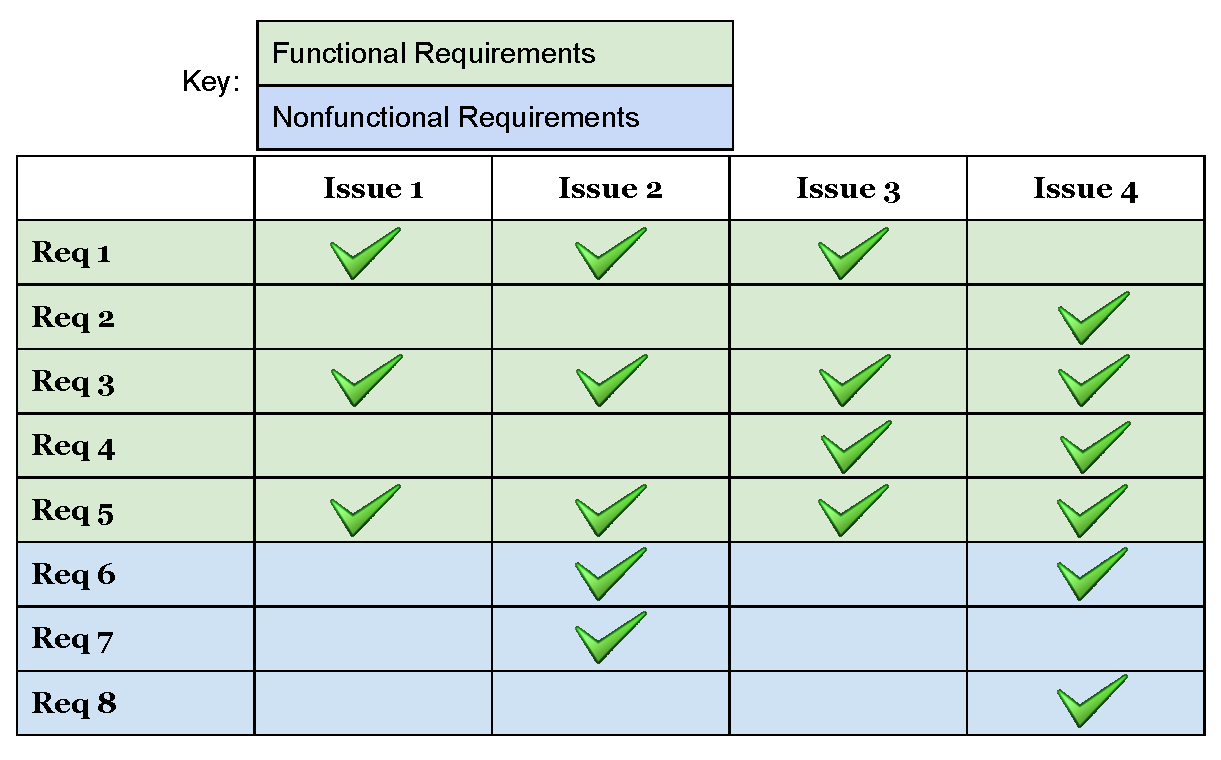
\includegraphics[width=1\textwidth]{images/issues_to_req_matrix.pdf}
  \caption{Matrix of project requirements to the issues this project attempts to
address}
\end{figure}
